\documentclass{article}
\usepackage{graphicx}

\author{Michael Fulton and David Josephs}
\date{April 29, 2015}
\title{Writeup For Assignment 2: BST, AVL, and Splay Trees}

\begin{document}
	\maketitle

	\section*{Status of Code}
		The implementation of Binary Search Trees is complete.  Insertion, searching, and removal all work as expected.  The implementation of AVL Trees still has several issues related to rotations, 
		including an error where during a rotation, part of the tree is copied and remains linked to by some elements, but forgotten by others.  There is also an issue which causes search to fail due to
		some pointers being misdirected (potentially related to the first issue).  Splay Trees are also implemented fully, but have some errors involving removal of a node with two children.

		This current state of the code means that the following answers and plots are based on the actual performance of BST (the plot is the actual performance of splay trees), and the expected performance of
		AVL trees and Splay trees (except for the plot, which has actual data from AVL trees);

	\section*{Analysis and Plot}
		\begin{enumerate}
			\item False. The worst case performance is O(N), but since the height of BST's average around O(log N), its operations average at O(log N).
			\item True. This should be the case, as all tree operations are a function of their height, and the AVL balancing (when working properly), should limit tree height to O(log N).
			\item True. This should be the case due to the nature of the average height of a splay tree, which comes out around O(log N).
		\end{enumerate}

		This following plot contains actual data from BST and Splay Tree implementations, and theoretical data from AVL trees.
		\clearpage
		
		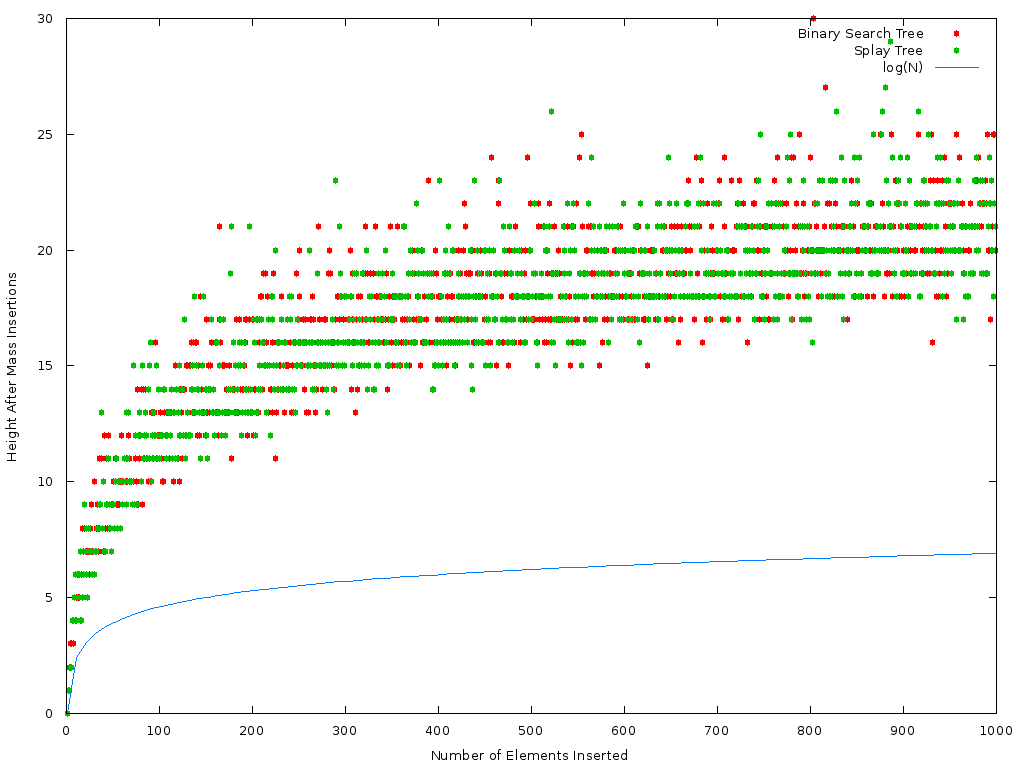
\includegraphics[scale = 0.7]{plot.png}
		
\end{document}
